% ====================================================================
% graphite_ica_ch1_v8-01.tex — Chapter 1 (v8-01: 유도 과정 교과서 확장판)
%   베이스 구조 = v7-11(절 순서·결과 박스·그림 5개·표·부호 사슬 보존).
%   확장 = 각 결과 박스마다 출발식→연산→중간식→박스 단계별 유도 복원
%   (AUTHOR_BRIEF_v8 §3 의 11식 유도 사슬 전부 가시화).
%   그림: v7-11 5개 체리픽(spine·staging·hysloop·logistic·reversal) +
%          신규 3개(g(ξ) 이중웰·V_eq 비단조·지연 ODE 완화).
%   부호: AUTHOR_BRIEF_v8 §7 의 8항 전수 검산 통과.
%   build: xelatex -interaction=nonstopmode 2-pass (kotex).
% ====================================================================
\documentclass[11pt,a4paper]{article}
\usepackage[margin=22mm]{geometry}
\usepackage{kotex}
\setmonofont{D2Coding}[Scale=MatchLowercase]
\usepackage{amsmath,amssymb,mathtools,bm}
\usepackage{booktabs,longtable,array}
\usepackage{enumitem}
\usepackage{amsthm}
\usepackage{hyperref}
\usepackage{fancyhdr}
\usepackage{lastpage}
\usepackage{setspace}
\usepackage{tikz}
\usetikzlibrary{positioning,arrows.meta,calc,fit,backgrounds}
\setstretch{1.12}
\setlength{\parskip}{0.45em}\setlength{\parindent}{0pt}\setlength{\headheight}{14pt}
\setlength{\emergencystretch}{2em}
\hypersetup{colorlinks=true, linkcolor=blue, urlcolor=blue, citecolor=blue,
  pdftitle={흑연 음극 dQ/dV 이론: 코드 진행 수식-구동 교과서판 — Chapter 1 (v8)}}
\pagestyle{fancy}\fancyhf{}
\lhead{흑연 음극 $dQ/dV$ 이론 — Ch.1 (v8, 유도 과정 교과서 확장판)}\rhead{\thepage/\pageref{LastPage}}
\renewcommand{\headrulewidth}{0.4pt}

\newtheorem*{keybox}{핵심}
\newtheorem*{codebox}{코드 대응}
\newtheorem*{signbox}{부호 검산}
\newtheorem*{verifybox}{검산}
\newtheorem*{derivebox}{유도}

\newcommand{\dd}{\mathrm{d}}
\newcommand{\eff}{\mathrm{eff}}
\newcommand{\eq}{\mathrm{eq}}
\newcommand{\app}{\mathrm{app}}
\newcommand{\cell}{\mathrm{cell}}
\newcommand{\bg}{\mathrm{bg}}
\newcommand{\rxn}{\mathrm{rxn}}
\newcommand{\dis}{\mathrm{dis}}
\newcommand{\chg}{\mathrm{chg}}
\newcommand{\hys}{\mathrm{hys}}
\newcommand{\work}{\mathrm{work}}
\newcommand{\rep}{\mathrm{rep}}
\newcommand{\lag}{\mathrm{lag}}
\newcommand{\sstat}{\mathrm{ss}}
\newcommand{\tot}{\mathrm{tot}}
\newcommand{\tail}{\mathrm{tail}}
\newcommand{\target}{\mathrm{target}}
\newcommand{\code}[1]{\texttt{#1}}

\renewcommand{\theequation}{1.\arabic{equation}}
\renewcommand{\thesection}{1.\arabic{section}}
\title{\textbf{\LARGE Chapter 1}\\[0.35em]\Large 흑연 음극 $dQ/dV$ 이론: 코드 진행을 따라가는 수식-구동 교과서 확장판}
\author{}
\date{}

\makeatletter
\renewcommand*\l@section[2]{%
  \ifnum \c@tocdepth >\z@
    \addpenalty\@secpenalty
    \addvspace{1.0em \@plus\p@}%
    \setlength\@tempdima{2.3em}%
    \begingroup
      \parindent \z@ \rightskip \@pnumwidth
      \parfillskip -\@pnumwidth
      \leavevmode \bfseries
      \advance\leftskip\@tempdima
      \hskip -\leftskip
      #1\nobreak\hfil
      \nobreak\hb@xt@\@pnumwidth{\hss #2\kern-\p@\kern\p@}\par
    \endgroup
  \fi}
\renewcommand*\l@subsection{\@dottedtocline{2}{2.3em}{3.2em}}
\makeatother

\begin{document}
\maketitle

% ====================================================================
\section*{서론 — 이 문건이 따라가는 것}
\addcontentsline{toc}{section}{서론}
% ====================================================================
리튬이온전지 흑연 음극의 incremental capacity analysis(ICA)는 충방전 곡선 $Q(V)$ 의 미분
$\dd Q/\dd V$ 를 본다 \cite{bloom2005,dubarry2012}. 흑연은 staging 상전이(stage
$4\!\to\!3\!\to\!2\mathrm L\!\to\!2\!\to\!1$)를 거치며 \cite{dahn1991,ohzuku1993}, 각 전이 전위에서
두 상이 공존하면 전위가 거의 평탄해 좁은 $\dd V$ 에 큰 $\dd Q$ 가 몰려 $\dd Q/\dd V$ 가 치솟는다.

본 문건은 이 곡선을 \emph{한 번 그리는 계산}을 그대로 따라간다. 계산은 구현
\code{Anode\_Fit\_v11\_final.py} 의 메서드 \code{dqdv} 한 번 호출이며, 그 내부는 아홉 단계
$\mathrm N0\!\to\!\mathrm N9$ 를 순서대로 밟는다(그림~\ref{fig:spine}). 각 절은 그 한 단계에서
코드가 평가하는 물리식을, \textbf{출발 전제 $\to$ 적용 연산 $\to$ 중간식 $\to$ 결과 박스}의 단계별 유도로 닫는다 — 학부생이 손으로 따라갈 수 있는 교과서 수준의 유도가 목표다.

\textbf{관측.}
\begin{quote}\itshape
$\dd Q/\dd V$ 상전이 peak 의 위치$\cdot$너비$\cdot$높이는 (a) 온도 $T$, (b) 극판 전위, (c) C-rate(전류)
세 가지에 따라 변한다. 저온$\cdot$고율일수록 peak 의 꼬리가 길어져 다음 peak 와 겹치고, 같은 전이가 충전과 방전에서
서로 다른 전위에 peak 를 남기며(충방전 히스테리시스), 이 갈림에는 전류를 $0$ 으로 줄여도 사라지지 않는 성분이 있다.
\end{quote}

세 인자는 모두 하나의 속도식 $k\simeq k_0\exp[-\Delta G_a/RT]$ 의 서로 다른 자리로 들어온다 — 온도는 지수의 분모,
전위는 장벽 $\Delta G_a$ 자체, C-rate 는 요구 속도와 공급 속도의 경쟁이다. 코드 진행이 이 세 갈래를 차례로 닫는다.

\begin{figure}[t]
\centering
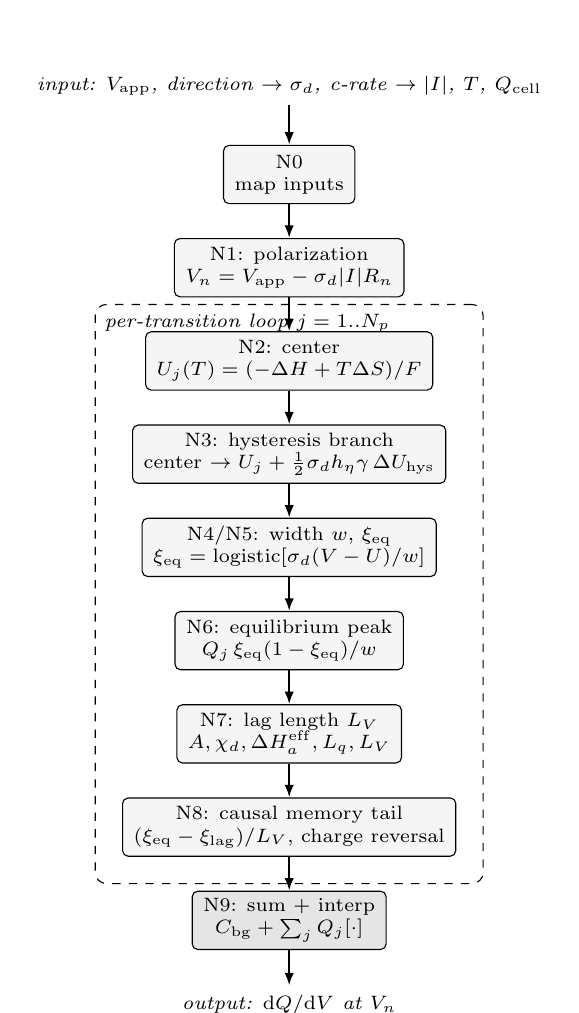
\begin{tikzpicture}[
  node distance=4.3mm and 5.5mm,
  stage/.style={draw,rounded corners=2pt,minimum height=7.4mm,inner xsep=4pt,inner ysep=2.5pt,font=\scriptsize,align=center,fill=black!4},
  core/.style={stage,fill=black!10},
  io/.style={font=\scriptsize\itshape,align=center},
  ar/.style={-{Latex[length=1.6mm]},thick}]
% input row
\node[io] (in) {input: $V_\app$, direction $\to\sigma_d$, c-rate $\to|I|$, $T$, $Q_\cell$};
% spine
\node[stage,below=5mm of in] (n0) {N0\\map inputs};
\node[stage,below=of n0] (n1) {N1: polarization\\$V_n=V_\app-\sigma_d|I|R_n$};
\node[stage,below=of n1] (n2) {N2: center\\$U_j(T)=(-\Delta H+T\Delta S)/F$};
\node[stage,below=of n2] (n3) {N3: hysteresis branch\\center $\to U_j+\tfrac12\sigma_d h_\eta\gamma\,\Delta U_\hys$};
\node[stage,below=of n3] (n4) {N4/N5: width $w$, $\xi_\eq$\\$\xi_\eq=\mathrm{logistic}[\sigma_d(V-U)/w]$};
\node[stage,below=of n4] (n6) {N6: equilibrium peak\\$Q_j\,\xi_\eq(1-\xi_\eq)/w$};
\node[stage,below=of n6] (n7) {N7: lag length $L_V$\\$A,\chi_d,\Delta H_a^\eff,L_q,L_V$};
\node[stage,below=of n7] (n8) {N8: causal memory tail\\$(\xi_\eq-\xi_\mathrm{lag})/L_V$, charge reversal};
\node[core,below=of n8] (n9) {N9: sum + interp\\$C_\bg+\sum_j Q_j[\cdot]$};
\node[io,below=4.5mm of n9] (out) {output: $\dd Q/\dd V$ at $V_n$};
\foreach \a/\b in {in/n0,n0/n1,n1/n2,n2/n3,n3/n4,n4/n6,n6/n7,n7/n8,n8/n9,n9/out}
  \draw[ar] (\a) -- (\b);
% per-transition loop bracket
\begin{scope}[on background layer]
\node[draw,dashed,rounded corners,fit=(n2)(n3)(n4)(n6)(n7)(n8),inner sep=3.4mm,label={[font=\scriptsize\itshape,anchor=north west]north west:per-transition loop $j=1..N_p$}] (loop) {};
\end{scope}
\end{tikzpicture}
\caption{한 곡선을 그리는 코드 진행(spine). 외부 실험조건이 \code{curve} facade 에서 $(\sigma_d,|I|,T,Q_\cell)$
로 환산($\mathrm N0$)되어 코어 \code{dqdv} 로 들어가고, 분극으로 내부 전위 $V_n$ 을 얻은 뒤($\mathrm N1$),
전이 $j$ 마다 평형 중심$\cdot$히스 분기$\cdot$폭$\cdot$평형 점유$\cdot$평형 peak$\cdot$지연 길이$\cdot$인과 꼬리를
계산해($\mathrm N2$--$\mathrm N8$) 합산$\cdot$역보간한다($\mathrm N9$). 본 문건의 절 번호가 이 노드 순서다.
점선 상자가 코드의 전이 루프(\code{for tr in transitions}).}
\label{fig:spine}
\end{figure}

\tableofcontents
\newpage

% ====================================================================
\section{기호와 규약, 실험조건 매핑 (N0)}\label{sec:notation}
% ====================================================================
계산의 진입점은 facade \code{curve}$(V_\app,\text{direction},\text{c\_rate},Q_\cell,T)$ 이고, 그 첫 일은 실험조건을
코어 \code{dqdv} 의 모델 입력으로 환산하는 것이다 — 이것이 노드 $\mathrm N0$ 다. 방향 문자열은 방향 부호 $\sigma_d$ 로,
C-rate 는 전류 크기 $|I|$ 로 바뀐다:
\begin{equation}
\sigma_d=\begin{cases}+1 & \text{방전(discharge)}\\ -1 & \text{충전(charge)}\end{cases},
\qquad
|I|=\text{c\_rate}\cdot Q_\cell\quad(\text{또는 }I_\mathrm{abs}\text{ 직접 지정}).
\label{eq:n0map}
\end{equation}
방향 부호의 작용처는 셋 — 분극 부호($\mathrm N1$), 분기 중심 선택($\mathrm N3$), 꼬리 지지 방향($\mathrm N8$) — 이며,
평형 종 자체는 방향 불변이다(아래에서 식으로 회수). 본 장이 뽑는 양은 $\dd Q/\dd V$ 한 곡선이다.

\textbf{전이 인덱스.} $j=1,\dots,N_p$($N_p\approx3$--$4$). 전이 $j$ 의 진행률 $\xi_j$(방전 시 $0\to1$ 로 증가, 곧 탈리튬화 진행),
용량 가중 $Q_j$. 박스 결과식은 $j$ 첨자를 단다.

\textbf{부호 규약(★최우선 결함 클래스).} 전위는 흑연 음극 반쪽전지 전위(vs Li/Li$^+$)다. 방향 부호 $\sigma_d=\pm1$
(방전 $+1$/충전 $-1$)이 코드의 \code{s} 인자이며, 평형 점유 $\xi_\eq=\mathrm{logistic}[\sigma_d(V-U)/w]$ 에서 방전
($\sigma_d=+1$)은 $V\!\uparrow\Rightarrow\xi_\eq\!\uparrow$(전위를 올리면 탈리튬화). 분기 중심 $\pm\tfrac12\sigma_d(\cdots)$
는 방전$\cdot$충전이 반대로 갈리고, 꼬리는 충전에서 격자 역전을 받는다.

\begin{longtable}{p{0.17\textwidth} p{0.16\textwidth} p{0.585\textwidth}}
\toprule 기호(코드 식별자) & 단위 & 의미 \\ \midrule \endhead
\multicolumn{3}{l}{\emph{— 실험조건$\cdot$방향(N0$\cdot$N1) —}}\\
$\sigma_d$ (\code{s},\,\code{sigma\_d}) & --- & 방향 부호 — 방전 $+1$/충전 $-1$ \\
$|I|$ (\code{I\_abs}) & A & 전류 크기 $=$ c\_rate$\cdot Q_\cell$ \\
$Q_\cell$ (\code{Q\_cell}) & C & 셀 용량(전하); $q=Q/Q_\cell$ 환산$\cdot$$|I|$ 환산 공용 \\
$T$ (\code{T}) & K & 온도 — 스칼라(등온) 또는 $V_\app$ 길이 배열($T(V)$ 비등온) \\
$R_n$ (\code{Rn}) & $\Omega$ & 음극 lumped 분극 저항 \\
$V_\app$ (\code{V\_app}) & V & 인가(측정) 전위 격자 \\
$V_n$ & V & 내부(열역학) 전위 $=V_\app-\sigma_d|I|R_n$ \\
\multicolumn{3}{l}{\emph{— 평형 중심$\cdot$폭$\cdot$점유(N2$\cdot$N4$\cdot$N5) —}}\\
$U_j(T)$ (\code{U},\,\code{func\_U\_j}) & V & 전이 $j$ 평형 중심 전위 $=(-\Delta H_\rxn+T\Delta S_\rxn)/F$ \\
$\Delta H_{\rxn,j},\Delta S_{\rxn,j}$ (\code{dH\_rxn},\code{dS\_rxn}) & {\footnotesize J/mol;\,J/(mol\,K)} & 삽입 \emph{반응} 엔탈피$\cdot$엔트로피(평형 — \emph{활성화}와 다름) \\
$n_j$ (\code{n}) & --- & 폭 다중도($w=n_jRT/F$; \code{w} 주면 $n=wF/RT$ 역산) \\
$w_j$ (\code{func\_w}/\code{func\_w\_eff}) & V & 전이 폭 척도 $=n_jRT/F$(옵션 $w^\eff$) \\
$\xi_{\eq,j}$ (\code{func\_ksi\_eq}) & --- & 평형 진행률(logistic) \\
$Q_j$ (\code{Q}) & C & 전이 $j$ 용량 가중 \\
$C_\bg$ (\code{Cbg}) & C/V & 배경 미분용량(상수 또는 $V$ 함수) \\
\multicolumn{3}{l}{\emph{— 히스테리시스 분기(N3) —}}\\
$\Omega_j$ (\code{Omega}) & J/mol & 정규용액 상호작용 에너지($>2RT$ 면 상분리$\cdot$히스) \\
$\gamma_j$ (\code{gamma}) & --- & 분기 축소 인자 $0\le\gamma_j\le1$($0$ 이면 분기 없음) \\
$\Delta U_j^\hys$ (\code{func\_dU\_hys}) & V & spinodal 상한 분기 gap \\
$h_{\eta,j}$ (\code{h\_eta}) & --- & 부분 cycle 인자(기본 $1$) \\
$U_j^{\,d}$ (\code{center},\,\code{func\_U\_branch}) & V & 방향별 분기 중심 \\
\multicolumn{3}{l}{\emph{— 동역학 꼬리(N7$\cdot$N8) —}}\\
$\chi$ (\code{chi},\,\code{x}) & --- & 전이상태 분율 위치(전달 계수); 방향별 $\chi_d$ \\
$\chi_d$ (\code{func\_chi\_d}) & --- & 방향별 전달 계수 — 방전 $\chi$/충전 $1-\chi$ \\
$\mathcal A$ (\code{A}) & J/mol & 꼬리 컷점 affinity $=\min(z_\mathrm{cut}n_jRT,\,A_\mathrm{cap}RT)$ \\
$\Delta H_{a,j},\Delta S_{a,j}$ (\code{dH\_a},\code{dS\_a}) & {\footnotesize J/mol;\,J/(mol\,K)} & \emph{활성화} 엔탈피$\cdot$엔트로피(속도) \\
$\Delta H_{a,j}^\eff$ (\code{func\_dH\_a\_eff}) & J/mol & 유효 장벽 $=\Delta H_a-\chi_d\Omega$ \\
$L_{q,j}$ (\code{func\_L\_q}) & --- & 용량축 지연 길이 \\
$L_{V,j}$ (\code{lag\_len\_V}) & V & 전압축 지연 길이 $=|\dd V/\dd q|_{q_a}L_{q,j}$ \\
$|\dd V/\dd q|_{q_a}$ (\code{dVdq\_qa}) & V & 컷점 OCV 기울기($L_q\to L_V$ 환산) \\
$z_\mathrm{cut}$ (\code{z\_cut}) & --- & 컷 affinity 의 $z=\mathcal A/(n_jRT)$(기본 $4.357$) \\
$A_\mathrm{cap}$ (\code{A\_cap\_RT}) & --- & 컷 affinity 상한 배수(기본 $4.0$) \\
$\xi_{\mathrm{lag},j}$ (\code{occ\_lagged}) & --- & 인과 저역통과된 진행률 \\
\multicolumn{3}{l}{\emph{— 상수 —}}\\
$R,F,k_B,h$ & {\footnotesize J/(mol\,K), C/mol, J/K, J\,s} & 기체상수, Faraday, Boltzmann, Planck \\
\bottomrule
\end{longtable}

흑연 staging 의 갤러리 채움을 그림~\ref{fig:staging} 에 둔다 — 각 stage 전이가 한 peak 를 남기고, 코드의 전이 리스트
\code{GRAPHITE\_STAGING\_LIT}(4건)이 이 네 전이의 초기값이다.

\begin{figure}[t]
\centering
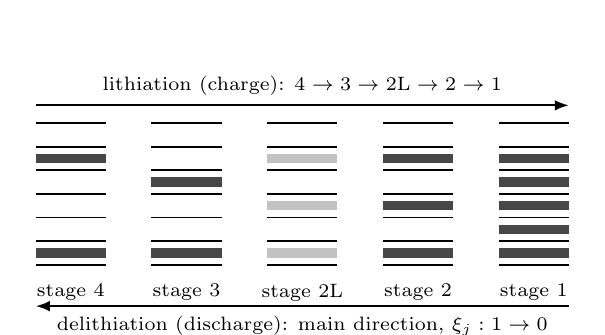
\begin{tikzpicture}[x=1.05cm,y=0.5cm,
  lab/.style={font=\scriptsize,align=center},
  fill4/.style={fill=black!72},fillL/.style={fill=black!24}]
% five stage columns, each shows graphene layers (lines) and Li-filled galleries (bands)
\def\colw{0.85}
% stage 4: 1 filled gallery of 4
\foreach \x/\name/\filled/\style in {0/{stage 4}/{1}/fill4, 1.4/{stage 3}/{1}/fill4, 2.8/{stage 2L}/{all}/fillL, 4.2/{stage 2}/{all}/fill4, 5.6/{stage 1}/{dense}/fill4}{
  \draw[semithick] (\x,0)--(\x+\colw,0);
  \foreach \k in {1,2,3,4,5,6}{\draw[semithick] (\x,0.6*\k)--(\x+\colw,0.6*\k);}
  \node[lab,below] at (\x+\colw/2,-0.25) {\name};
}
% stage 4: every 4th gallery filled
\foreach \k in {1,5}{\fill[black!72] (0,0.6*\k-0.42) rectangle (0+\colw,0.6*\k-0.18);}
% stage 3: every 3rd
\foreach \k in {1,4}{\fill[black!72] (1.4,0.6*\k-0.42) rectangle (1.4+\colw,0.6*\k-0.18);}
% stage 2L: every 2nd, light (liquid-like)
\foreach \k in {1,3,5}{\fill[black!24] (2.8,0.6*\k-0.42) rectangle (2.8+\colw,0.6*\k-0.18);}
% stage 2: every 2nd, dark
\foreach \k in {1,3,5}{\fill[black!72] (4.2,0.6*\k-0.42) rectangle (4.2+\colw,0.6*\k-0.18);}
% stage 1: all galleries
\foreach \k in {1,2,3,4,5}{\fill[black!72] (5.6,0.6*\k-0.42) rectangle (5.6+\colw,0.6*\k-0.18);}
\draw[-{Latex[length=1.8mm]},thick] (0,4.05)--(6.45,4.05) node[pos=0.5,above,font=\scriptsize] {lithiation (charge): $4\to3\to2\mathrm L\to2\to1$};
\draw[{Latex[length=1.8mm]}-,thick] (0,-1.05)--(6.45,-1.05) node[pos=0.5,below,font=\scriptsize] {delithiation (discharge): main direction, $\xi_j:1\to0$};
\end{tikzpicture}
\caption{흑연 staging 의 갤러리 채움 도식(v7-11 유래). 수평선이 그래핀 층, 음영 띠가 리튬이 든 층간 갤러리다.
채울수록 stage 번호가 줄어 stage 1($\mathrm{LiC_6}$, 완전 채움)에 닿고, 각 stage 전이가 $\dd Q/\dd V$ 에 peak
하나를 남긴다. stage $2\mathrm L$ 은 면내 질서가 풀린 단계라 옅게 표시했다. 코드의 전이 리스트 4건이 이 전이들의
초기값이다.}
\label{fig:staging}
\end{figure}

% ====================================================================
\section{분극 — 측정 전위에서 내부 전위로 (N1)}\label{sec:pol}
% ====================================================================
코어 \code{dqdv} 의 첫 식은 분극을 벗기는 환산이다. 관측은 유한 전류에서 이루어지므로 측정 전위 $V_\app$ 에는 셀의
직렬 저항을 통과한 IR 분극이 실려 있고, 평형 열역학이 사는 전위는 그 분극을 벗긴 내부 전위 $V_n$ 이다.

\subsection{분극 부호 — 방향이 결정한다}
전류 크기 $|I|$ 가 lumped 저항 $R_n$ 을 통과하며 만드는 전위 강하가 $|I|R_n$ 이고, 그 부호는 전류 방향이 정한다.
방전($\sigma_d=+1$)은 음극에서 산화(탈리튬화)가 일어나는 방향이라 측정 전위가 내부 전위보다 분극만큼 \emph{높게}
관측되므로, 내부 전위는 그만큼 낮춰 읽어야 한다. 충전($\sigma_d=-1$)은 부호가 반대다. 두 경우를 한 식으로 묶으면
\begin{equation}
\boxed{\;V_n\;=\;V_\app\;-\;\sigma_d\,|I|\,R_n\;.}
\label{eq:vn}
\end{equation}
이것이 코드의 \code{V\_n = V\_in - sigma\_d * I\_abs * self.Rn} 한 줄이다. 부호 약속을 식으로 확인하면 —
방전에서 $V_n=V_\app-|I|R_n<V_\app$(측정이 내부보다 높음), 충전에서 $V_n=V_\app+|I|R_n>V_\app$ — 이며,
$|I|\to0$ 또는 $R_n=0$ 에서 $V_n=V_\app$ 로 두 전위가 일치한다.

\subsection{작업 격자 — 꼬리가 들어올 여유}
이후 모든 전이 계산은 $V_n$ 을 직접 쓰지 않고, $V_n$ 의 범위를 양쪽으로 넓힌 균일 \emph{작업 격자} $V_\work$ 위에서
이루어진다. 넓힘은 동역학 꼬리(\S\ref{sec:tail})가 격자 밖에서 잘려 인공 절단이 생기지 않도록 하는 여유다.
$v_\mathrm{lo}=\min V_n$, $v_\mathrm{hi}=\max V_n$, $\Delta v=v_\mathrm{hi}-v_\mathrm{lo}$ 로
\begin{equation}
V_\work=\mathrm{linspace}\big(v_\mathrm{lo}-p_\mathrm{lo}\,\Delta v,\;
v_\mathrm{hi}+p_\mathrm{hi}\,\Delta v,\;n_\work\big),
\qquad \Delta_\mathrm{grid}=V_{\work,1}-V_{\work,0},
\label{eq:vwork}
\end{equation}
패딩 $p_\mathrm{lo}=p_\mathrm{hi}=0.15$, 점 수 $n_\work=\max(2048,\,2\,|V_n|)$ 이다(코드 \code{grid\_pad\_lo/hi},
\code{n\_work\_min}). 온도가 배열 $T(V)$ 이면 같은 격자 위로 보간해 $T_\work$ 를 얻고($T_\mathrm{rep}=\overline{T_\work}$ 는
전이당 상수 평가용 대표 온도), 스칼라면 $T_\work\equiv T$ 다. 배경은 작업 격자 위에서 먼저 깔린다:
$\dd Q/\dd V|_\work \leftarrow C_\bg(V_\work)$. 모든 전이 기여는 여기에 더해지고($\mathrm N9$), 마지막에 $V_n$ 으로
역보간된다.

\begin{keybox}
\textbf{세 전위.} $V_\app$(측정)$\cdot$$V_n$(내부, 식~\eqref{eq:vn})$\cdot$$V_\work$(계산 격자, 식~\eqref{eq:vwork})는
지위가 다르다. 다음 절부터 평형$\cdot$동역학은 $V_\work$ 위에서 풀고, 출력만 $V_n$ 으로 되돌린다.
\end{keybox}

다음 절은 전이 루프의 첫 식 — 평형 중심 $U_j(T)$ — 으로 들어간다.

% ====================================================================
\section{평형 중심 $U_j(T)$ — 열역학에서 (N2)}\label{sec:center}
% ====================================================================
전이 루프 안의 첫 물리량은 전이 $j$ 의 평형 중심 전위 $U_j(T)$ 다. 코드는 이를 열역학 입력 $(\Delta H_\rxn,\Delta S_\rxn)$
에서 \code{func\_U\_j} 로 계산하거나(없으면) \code{'U'} 를 직접 읽는다. 이 절은 그 환산식이 어디서 오는지를 닫는다.

\subsection{$G$ 와 $\mu$ — 등온$\cdot$등압 열역학의 언어}
등온$\cdot$등압 계(전지)의 자발성$\cdot$평형을 판정하는 퍼텐셜은 Gibbs 자유에너지다:
\begin{equation}
G\;\equiv\;H-TS.
\label{eq:gibbsdef}
\end{equation}
자발 변화는 $G$ 감소 방향, 평형은 $G$ 극소다. 입자 1몰 변화당 $G$ 변화가 화학퍼텐셜이다:
\begin{equation}
\mu\;\equiv\;\frac{\partial G}{\partial n}\bigg|_{T,P}.
\label{eq:mudef}
\end{equation}
입자는 $\mu$ 높은 곳에서 낮은 곳으로 흐르고, 두 장소의 $\mu$ 일치가 입자 교환 평형이다.

\subsection{삽입 반응의 전기화학 평형}
삽입 반응 $\mathrm{Li}^++e^-+[\,]\rightleftharpoons\mathrm{Li}_{(\text{흑연})}$ 에서 리튬은 $\mathrm{Li}^+$ 와 $e^-$ 로 갈라져 드나든다.
전자 항에는 측정 전위 $V$ 를 통해 전기 일 $(-1)\cdot F\cdot(-V)=FV$ 가 더해진다. 반응 1몰당 자유에너지 변화는
\begin{equation}
\Delta G_j\;=\;G_{\mathrm{Li}_{(\text{그래핀})}}\;-\;G_{\mathrm{Li}^+}\;-\;G_{e^-}\;-\;G_{[\,]}.
\label{eq:dGreaction}
\end{equation}
전극 내 전위 $V$ 가 전자 항에 $-FV$ 로 들어오므로($e^-$ 의 전기화학 퍼텐셜 $=\mu_{e^-}^0-FV$), 전기화학 평형 조건
$\Delta G_j=0$ 은 전위 의존으로:
\begin{equation}
\mu_\mathrm{Li}(\xi_\eq)\;=\;\mu^0\;-\;sF\,(V-U_j),
\qquad \Delta G_j\;=\;-sF\,U_j
\label{eq:eqcond}
\end{equation}
형태가 된다($s=+1$; $U_j$ 는 비배치 몫 자유에너지의 전위 환산). 즉 $\Delta G_j=-sFU_j$ 이다.

\subsection{$U_j(T)$ 의 유도}
\begin{derivebox}
\textbf{출발: Gibbs 항등식.} $\Delta G_j=\Delta H_{\rxn,j}-T\Delta S_{\rxn,j}$ (등압 등온 반응).

\textbf{대입: } 위 식~\eqref{eq:eqcond} 의 $\Delta G_j=-sF\,U_j$ ($s=+1$)에 대입한다:
\begin{equation*}
-F\,U_j\;=\;\Delta H_{\rxn,j}-T\,\Delta S_{\rxn,j}.
\end{equation*}

\textbf{$U_j$ 에 대해 풀기:} 양변을 $-F$ 로 나누면
\end{derivebox}
\begin{equation}
\boxed{\;U_j(T)\;=\;\frac{-\Delta H_{\rxn,j}+T\,\Delta S_{\rxn,j}}{F}\;.}
\label{eq:Uj}
\end{equation}
이것이 \code{func\_U\_j(T, dH\_rxn, dS\_rxn)} 의 \code{(-dH\_rxn + T*dS\_rxn)/F} 다.

\textbf{부호 독해.} 발열 반응 $\Delta H_\rxn<0$ 이면 분자 $-\Delta H_\rxn>0$ 이 중심을 \emph{올린다}(흡열 아님에 주의).
온도 의존은 $\partial U_j/\partial T=\Delta S_{\rxn,j}/F$ 이고, $|\Delta S_\rxn|\sim$ 수$\sim$수십 J/(mol\,K) 라
$30$ K 창에서 수 mV 규모로 중심이 이동한다 — 다온도 피팅에서 온도마다 $U_j(T)$ 를 따로 읽어야 하는 이유다.

\begin{codebox}
\textbf{N2.} \code{if 'dH\_rxn' in tr and 'dS\_rxn' in tr: U\_j = func\_U\_j(T\_work, dH\_rxn, dS\_rxn)}
— 배열 $T_\work$ 대응. 없으면 \code{U\_j = float(tr['U'])} 직접. \code{GRAPHITE\_STAGING\_LIT} 의 stage 2$\to$1 은
$\Delta H_\rxn=-13000$ J/mol, $\Delta S_\rxn=-16$ J/(mol\,K) $\Rightarrow$ $U(298)=(13000-298.15\times16)/96485
\approx0.0853$ V(목표 $0.085$ V 정합).
\end{codebox}

다음은 같은 루프 안에서 이 중심을 충$\cdot$방전으로 갈라놓는 히스테리시스 분기다.

% ====================================================================
\section{히스테리시스 분기 중심 (N3)}\label{sec:hys}
% ====================================================================
코드는 평형 중심 $U_j$ 를 곧바로 쓰지 않고, 상호작용 $\Omega_j$ 와 분기 인자 $\gamma_j$ 가 있으면 방향별 분기 중심
$U_j^{\,d}$ 로 옮긴다. 방전과 충전이 같은 전이를 서로 다른 준안정 가지로 과주행해 중심이 갈라지는 현상이다.

\subsection{자유에너지와 spinodal}
격자기체의 자유에너지를 진행률 $\xi=1-\theta$ 로 적으면 이상 섞임 엔트로피 몫과 정규용액 상호작용 몫이 더해진다:
\begin{equation}
g_j(\xi)=g_j^0+RT\big[\xi\ln\xi+(1-\xi)\ln(1-\xi)\big]+\Omega_j\,\xi(1-\xi).
\label{eq:gxi}
\end{equation}
$g_j''(\xi)=RT/[\xi(1-\xi)]-2\Omega_j$ 를 얻는다. $g_j''=0$ 의 두 근이 spinodal 이다:

\begin{derivebox}
\textbf{출발: } $g_j''(\xi)=\dfrac{RT}{\xi(1-\xi)}-2\Omega_j=0$.

\textbf{정리: } $\dfrac{RT}{\xi(1-\xi)}=2\Omega_j$ $\Longrightarrow$ $\xi(1-\xi)=\dfrac{RT}{2\Omega_j}$ $\Longrightarrow$
$\xi^2-\xi+\dfrac{RT}{2\Omega_j}=0$.

\textbf{근의 공식 적용: } $\xi=\dfrac{1\pm\sqrt{1-4\cdot RT/(2\Omega_j)}}{2}=\dfrac{1\pm\sqrt{1-2RT/\Omega_j}}{2}$.
\end{derivebox}

따라서 spinodal 두 근은
\begin{equation}
\xi_{s,j}^\pm=\tfrac12(1\pm u_j),\qquad
u_j\equiv\sqrt{1-\frac{2RT}{\Omega_j}}\quad(\Omega_j>2RT).
\label{eq:spinodal}
\end{equation}
$u_j$ 가 실수가 되는 조건 $\Omega_j>2RT$ 가 상분리(따라서 히스테리시스)의 문턱이다. $\Omega_j\le2RT$ 면 갈라짐이 없다.
이 문턱이 코드의 명시 분기 \code{if Omega <= 2RT: return 0.0} 이다.

\subsection{평형 전위 곡선의 비단조성과 과주행}
식~\eqref{eq:gxi} 를 진행률로 미분하면 자유에너지 기울기 $g_j'(\xi)=RT\ln[\xi/(1-\xi)]+\Omega_j(1-2\xi)$ 를 얻고,
이것이 평형 전위 함수 $V_{\eq,j}(\xi)=U_j+(1/sF)\cdot g_j'(\xi)$ 이므로:
\begin{equation}
V_{\eq,j}(\xi)=U_j+\frac{RT}{sF}\ln\frac{\xi}{1-\xi}+\frac{\Omega_j}{sF}(1-2\xi).
\label{eq:Veq}
\end{equation}
$\Omega_j>2RT$ 면 이 곡선이 비단조다(그림~\ref{fig:hysloop}). 방전은 $\xi\!\approx\!0$ 에서 상승 가지를 극대
$\xi_{s,j}^-$ 까지, 충전은 $\xi\!\approx\!1$ 에서 극소 $\xi_{s,j}^+$ 까지 과주행한다(그림~\ref{fig:hysloop}).

\begin{figure}[t]
\centering
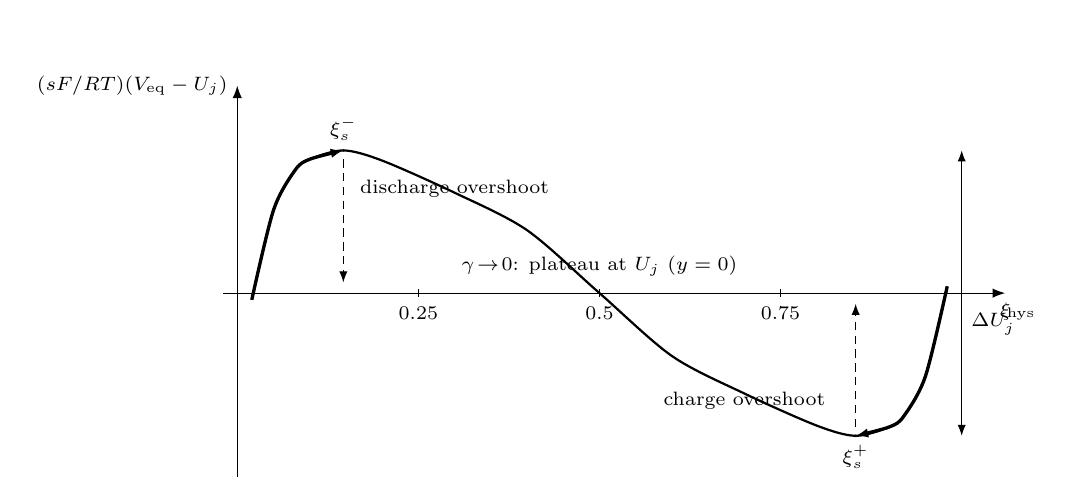
\begin{tikzpicture}[x=9.2cm,y=1.7cm]
\draw[-{Latex[length=1.6mm]}] (0,-1.45) -- (0,1.55) node[left,font=\scriptsize] {$(sF/RT)(V_\eq-U_j)$};
\draw[-{Latex[length=1.6mm]}] (-0.02,0) -- (1.06,0) node[below,font=\scriptsize] {$\xi$};
\foreach \xx in {0.25,0.5,0.75} {\draw (\xx,0.03) -- (\xx,-0.03) node[below,font=\scriptsize] {\xx};}
% non-monotone V_eq(xi) for Omega=4RT (qualitative)
\draw[thick] plot[smooth] coordinates {(0.02,-0.05) (0.05,0.62) (0.08,0.92) (0.1,1.00) (0.1464,1.066) (0.2,0.99) (0.3,0.75) (0.4,0.47) (0.5,0) (0.6,-0.47) (0.7,-0.75) (0.8,-0.99) (0.8536,-1.066) (0.9,-1.00) (0.92,-0.92) (0.95,-0.62) (0.98,0.05)};
\fill (0.1464,1.066) circle (0.5pt) node[above,font=\scriptsize] {$\xi_s^-$};
\fill (0.8536,-1.066) circle (0.5pt) node[below,font=\scriptsize] {$\xi_s^+$};
\draw[{Latex[length=1.4mm]}-{Latex[length=1.4mm]}] (1.0,-1.066) -- (1.0,1.066) node[pos=0.4,right,font=\scriptsize] {$\Delta U_j^\hys$};
% discharge overshoot path (rising branch up to xi_s^-)
\draw[-{Latex[length=1.6mm]},very thick] plot[smooth] coordinates {(0.02,-0.05) (0.05,0.62) (0.08,0.92) (0.1,1.00) (0.1464,1.066)};
\draw[-{Latex[length=1.4mm]},densely dashed] (0.1464,1.0) -- (0.1464,0.08);
\node[font=\scriptsize] at (0.30,0.78) {discharge overshoot};
% charge overshoot path
\draw[-{Latex[length=1.6mm]},very thick] plot[smooth] coordinates {(0.98,0.05) (0.95,-0.62) (0.92,-0.92) (0.9,-1.00) (0.8536,-1.066)};
\draw[-{Latex[length=1.4mm]},densely dashed] (0.8536,-1.0) -- (0.8536,-0.08);
\node[font=\scriptsize] at (0.70,-0.80) {charge overshoot};
\node[font=\scriptsize] at (0.5,0.20) {$\gamma\!\to\!0$: plateau at $U_j$ ($y=0$)};
\end{tikzpicture}
\caption{비단조 평형 전위 $V_\eq(\xi)$($\Omega_j=4RT$)와 과주행(v7-11 유래). 방전(굵은 경로, 좌상)은 극대 $\xi_s^-$ 까지,
충전(우하)은 극소 $\xi_s^+$ 까지 과주행해 중심이 갈라진다. 두 극값 차가 spinodal 상한 gap $\Delta U_j^\hys$
(식~\eqref{eq:dUhys}), 실측 분기는 $\gamma_j$ 만큼 안쪽(식~\eqref{eq:Ubranch}).}
\label{fig:hysloop}
\end{figure}

\subsection{$g(\xi)$ 이중웰 — 신규 그림}

\begin{figure}[t]
\centering
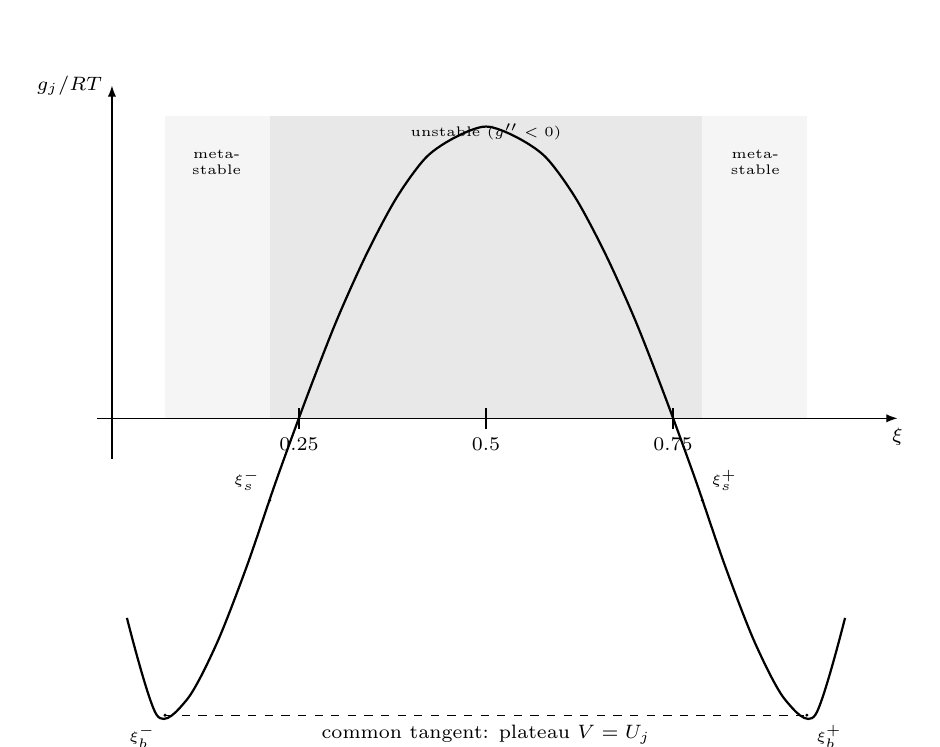
\begin{tikzpicture}[x=9.5cm,y=65cm]
% g(xi) double-well for Omega=3RT (computed): g = RT[xi ln xi + (1-xi)ln(1-xi)] + Omega*xi*(1-xi)
% subtract linear: g - g^0 - linear_fit, values are g/(RT) with Omega=3RT
% approximate: entropy min at edges, bump in middle (spinodal at 0.211/0.789)
\fill[gray!18] (0.211,0) rectangle (0.789,0.059);
\fill[gray!8] (0.071,0) rectangle (0.211,0.059);
\fill[gray!8] (0.789,0) rectangle (0.929,0.059);
\node[font=\tiny] at (0.5,0.056) {unstable ($g''<0$)};
\node[font=\tiny,align=center] at (0.14,0.050) {meta-\\stable};
\node[font=\tiny,align=center] at (0.86,0.050) {meta-\\stable};
\draw[-{Latex[length=1.4mm]}] (0,-0.008) -- (0,0.065) node[left,font=\scriptsize] {$g_j/RT$};
\draw[-{Latex[length=1.4mm]}] (-0.02,0) -- (1.05,0) node[below,font=\scriptsize] {$\xi$};
\foreach \xx in {0.25,0.5,0.75} {\draw (\xx,0.002) -- (\xx,-0.002) node[below,font=\scriptsize] {\xx};}
% g(xi)/RT - linear_envelope for Omega=3RT
\draw[thick] plot[smooth] coordinates {(0.02,-0.039) (0.06,-0.058) (0.1,-0.055) (0.14,-0.044) (0.18,-0.029) (0.22,-0.012) (0.26,0.004) (0.30,0.019) (0.34,0.032) (0.38,0.043) (0.42,0.051) (0.46,0.055) (0.50,0.057) (0.54,0.055) (0.58,0.051) (0.62,0.043) (0.66,0.032) (0.70,0.019) (0.74,0.004) (0.78,-0.012) (0.82,-0.029) (0.86,-0.044) (0.90,-0.055) (0.94,-0.058) (0.98,-0.039)};
% common tangent (flat at Omega=3RT, symmetric -> horizontal)
\draw[dashed] (0.071,-0.058) -- (0.929,-0.058) node[pos=0.5,below,font=\scriptsize] {common tangent: plateau $V=U_j$};
\fill (0.071,-0.058) circle (0.6pt) node[below left,font=\tiny] {$\xi_b^-$};
\fill (0.929,-0.058) circle (0.6pt) node[below right,font=\tiny] {$\xi_b^+$};
\fill (0.211,-0.016) circle (0.6pt) node[above left,font=\tiny] {$\xi_s^-$};
\fill (0.789,-0.016) circle (0.6pt) node[above right,font=\tiny] {$\xi_s^+$};
\end{tikzpicture}
\caption{자유에너지 $g_j(\xi)$($\Omega_j=3RT$)의 이중웰(신규). 진한 중앙 띠(spinodal 구간 $\xi_s^-$--$\xi_s^+$)는
$g''<0$ 으로 즉시 불안정, 옅은 두 띠(binodal--spinodal 사이)는 준안정 — 히스테리시스의 무대다. 두 접점 $\xi_b^\pm$
를 잇는 공통 접선(파선)이 plateau 전위 $U_j$ 에 해당하고, 좁은 $\dd V$ 에 큰 $\dd Q$ 가 몰리는 ICA peak 의 열역학적 정체다.}
\label{fig:doublewell}
\end{figure}

\subsection{$\Delta U_j^\hys$ 의 유도}
두 spinodal 끝점의 전위 차가 분기 gap 의 spinodal 상한이다.

\begin{derivebox}
\textbf{출발: } 평형 전위~\eqref{eq:Veq}: $V_{\eq,j}(\xi)=U_j+\dfrac{RT}{sF}\ln\dfrac{\xi}{1-\xi}+\dfrac{\Omega_j}{sF}(1-2\xi)$.

\textbf{spinodal 값~\eqref{eq:spinodal} 대입.} $\xi_{s,j}^\pm=\tfrac12(1\pm u_j)$ 를 각 항에:
\begin{alignat*}{2}
\frac{\xi_{s,j}^\pm}{1-\xi_{s,j}^\pm}&=\frac{1\pm u_j}{1\mp u_j},\qquad
&(1-2\xi_{s,j}^\pm)&=\mp u_j.
\end{alignat*}

\textbf{중간식 — 극대 전위:}
\begin{equation*}
V_{\eq,j}(\xi_{s}^-)=U_j+\frac{RT}{sF}\ln\frac{1-u_j}{1+u_j}+\frac{\Omega_j}{sF}\,u_j.
\end{equation*}
\textbf{중간식 — 극소 전위:}
\begin{equation*}
V_{\eq,j}(\xi_{s}^+)=U_j+\frac{RT}{sF}\ln\frac{1+u_j}{1-u_j}-\frac{\Omega_j}{sF}\,u_j.
\end{equation*}

\textbf{차 계산 (극대 $-$ 극소):} $U_j$ 상쇄 후
\begin{equation*}
\Delta U_j^\hys=\frac{RT}{sF}\bigg[\ln\frac{1-u_j}{1+u_j}-\ln\frac{1+u_j}{1-u_j}\bigg]
+\frac{2\Omega_j\,u_j}{sF}.
\end{equation*}
\textbf{중간식 — 로그 항:} $\ln(a)-\ln(1/a)=2\ln a$, 그리고
$\ln\dfrac{1-u}{1+u}=-2\,\mathrm{artanh}\,u$ ($\mathrm{artanh}\,u=\tfrac12\ln\tfrac{1+u}{1-u}$ 로부터),
따라서 $\ln\dfrac{1-u}{1+u}-\ln\dfrac{1+u}{1-u}=-4\,\mathrm{artanh}\,u$.

\textbf{정리:} $\Delta U_j^\hys=\dfrac{RT}{sF}(-4\,\mathrm{artanh}\,u_j)+\dfrac{2\Omega_j u_j}{sF}$
$=\dfrac{2}{sF}(\Omega_j u_j-2RT\,\mathrm{artanh}\,u_j)$.
\end{derivebox}

\begin{equation}
\boxed{\;\Delta U_j^\hys
=\frac{2}{F}\Big[\Omega_j\,u_j-2RT\,\mathrm{artanh}\,u_j\Big],
\qquad u_j=\sqrt{1-\frac{2RT}{\Omega_j}}\;.}
\label{eq:dUhys}
\end{equation}
($s=+1$; $\mathrm{artanh}\,u=\tfrac12\ln\tfrac{1+u}{1-u}$ 로 로그 항을 정리.) 이것이 \code{func\_dU\_hys(T, Omega)} 의
\code{(2/F)*(Omega*u - 2*R*T*arctanh(u))} 이며, $\Omega\le2RT$ 면 $0$ 을 반환한다(제곱근 NaN 영역의 명시 분기).

\textbf{부호.} 극대 $>$ 극소라 $\Delta U_j^\hys\ge0$ 이고, $\Omega_j\to2RT^+$ 에서 $u_j\to0$, $\Delta U_j^\hys\to0$ 으로
연속이다.

\subsection{방향별 분기 중심 $U_j^{\,d}$}
두 spinodal 끝점의 \emph{평균}은 $U_j$ 에 정확히 걸린다 — 분기는 $U_j$ 대칭이다. 이 대칭 위에서 실측 분기 중심을
방향별 한 자유도로 적으면
\begin{equation}
\boxed{\;U_j^{\,d}\;=\;U_j\;+\;\tfrac12\,\sigma_d\,h_{\eta,j}\,\gamma_j\,\Delta U_j^\hys\;.}
\label{eq:Ubranch}
\end{equation}
이것이 \code{func\_U\_branch(T, U\_j, Omega, gamma, sigma\_d, h\_eta)} 의
\code{U\_j + 0.5*sigma\_d*h\_eta*gamma*func\_dU\_hys(T, Omega)} 다. 방전($\sigma_d=+1$)은 중심을 $+$ 쪽,
충전($\sigma_d=-1$)은 $-$ 쪽으로 옮겨 $U_j^{\dis}>U_j^{\chg}$(방전 전위가 충전보다 높다는 관측 일치).

코드는 전이당 상수인 분기 shift 만 필요하므로, 식~\eqref{eq:Ubranch} 의 $U_j$ 자리에 $0$ 을 넣어 shift 분을 얻고,
배열 중심 $U_j$ 에 더한다:
\begin{equation}
\mathrm{center}=
\begin{cases}
U_j+\tfrac12\sigma_d h_{\eta,j}\gamma_j\Delta U_j^\hys(T_\rep) & \gamma_j\ne0 \text{ 이고 } \Omega_j>0\\[2pt]
U_j & \text{그 외(분기 없음)}.
\end{cases}
\label{eq:center}
\end{equation}
이 \code{center} 가 다음 절 평형 점유 $\xi_\eq$ 의 중심으로 들어간다.

% ====================================================================
\section{폭과 평형 점유 $\xi_\eq$ (N4, N5)}\label{sec:width}
% ====================================================================
중심이 정해지면 코드는 폭 $w_j$ 와 평형 점유 $\xi_{\eq,j}$ 를 평가한다.

\subsection{폭 $w_j$ — 이상 격자기체 극한}
이상 격자기체($\Omega_j=0$)에서 폭 척도는 $w_j=RT/F$ 이다. 폭 다중도 $n_j$ 는 여러 동등 자리가 한 전이를
이루는 일반화로, $n_j$ 가 다른 것은 격자기체 정지점 조건을 $n_j$ 개 자리에 대해 쓸 때 분모의 $RT/F$ 가
$n_j$ 배로 늘어나기 때문이다:
\begin{equation}
w_j=\frac{n_jRT}{F}\qquad(\text{기본 폭}).
\label{eq:wbase}
\end{equation}
코드 \code{func\_w(T, n)} 의 \code{n*R*T/F}
가 이것이고, 전이 dict 가 \code{'w'} 를 직접 주면 $n_j=w_jF/(RT)$ 로 역산해(\code{\_n\_factor}) 같은 식에 넣는다.
상호작용이 종을 좁히는 옵션 유효 폭은
\begin{equation}
w_j^\eff=\frac{RT}{F}\Big(1-\frac{\Omega_j}{2RT}\Big),
\label{eq:weff}
\end{equation}
이며 $\Omega_j\to2RT$ 에서 $0$ 으로 가므로 코드는 $\mathrm{floor\_frac}\cdot RT/F$ 하한으로 클립한다(\code{func\_w\_eff},
기본 \code{w\_eff\_floor\_frac}$=0.05$). 식~\eqref{eq:weff} 는 식~\eqref{eq:Veq} 의 중심($\xi=\tfrac12$) 기울기
$\dd V_{\eq}/\dd\xi|_{1/2}=(RT-2\Omega_j\cdot\xi(1-\xi))\cdot 1/(sF\cdot\xi(1-\xi))|_{1/2}=(4RT-2\Omega_j)/(sF)$ 에서
$4Fw_j^\eff=4RT-2\Omega_j$ 를 풀어 얻는다.

\subsection{평형 점유 $\xi_\eq$ — logistic 의 유도}
격자기체 운동방정식을 통해 평형이 logistic 으로 닫히는 과정을 단계별로 밟는다.

\textbf{구동력.} 전이 $j$ 의 구동력(affinity)은 전위 $V$ 가 평형 중심 $U_j^{\,d}$ 에서 벗어난 전기 항이다:
$\mathcal A_j=sF(V-U_j^{\,d})$.

\textbf{정$\cdot$역 속도.} 정방향(탈리튬화) 속도 $r_j^+=k_0 e^{-(\Delta G_a-\chi\mathcal A_j)/RT}$ 와 역방향
$r_j^-=k_0 e^{-(\Delta G_a+(1-\chi)\mathcal A_j)/RT}$ 의 비를 취하면 $\chi$ 가 상쇄되어
\begin{equation}
\frac{r_j^+}{r_j^-}=e^{\mathcal A_j/RT}
\label{eq:db}
\end{equation}
가 되는데, 이것이 detailed balance 조건이다. 운동방정식의 정지점 $r_j^+(1-\xi_j)=r_j^-\xi_j$ 에 식~\eqref{eq:db} 를 쓰면
\begin{equation}
\frac{\xi_{\sstat,j}}{1-\xi_{\sstat,j}}=\frac{r_j^+}{r_j^-}=e^{\mathcal A_j/RT}.
\label{eq:stationary}
\end{equation}

\begin{derivebox}
\textbf{logistic 풀기.} 구동력 $\mathcal A_j=sF(V-U_j^{\,d})$ 와 폭 $w_j=n_jRT/F$ 를 정의하면
$\mathcal A_j/RT=sF(V-U_j^{\,d})/(n_jRT/F\cdot F/F)=\sigma_d(V-U_j^{\,d})/w_j$ ($s=\sigma_d$).

\textbf{중간식.} $\xi/(1-\xi)=e^{\sigma_d(V-U_j^{\,d})/w_j}$ 에서 양변을 $e^z$ ($z\equiv\sigma_d(V-U_j^{\,d})/w_j$) 로 표기하면:
$\xi=e^z(1-\xi)$ $\Rightarrow$ $\xi(1+e^z)=e^z$ $\Rightarrow$ $\xi=e^z/(1+e^z)=1/(1+e^{-z})$.
\end{derivebox}

이 정지점은 detailed balance 가 열역학과 묶은 평형 그 자체이므로, $\xi_{\sstat}\to\xi_\eq$ 로 표기를 바꾸면
\begin{equation}
\boxed{\;\xi_{\eq,j}(V,T)=\frac{1}{1+\exp\!\big[-\sigma_d(V-U_j^{\,d})/w_j\big]}\;.}
\label{eq:xieq}
\end{equation}
폭 다중도 $n_j$ 는 식~\eqref{eq:wbase} 의 $w_j=n_jRT/F$ 로 logistic 인자의 분모에 들어간다.

\begin{signbox}
\textbf{부호.} 방전 $\sigma_d=+1$: $V\!\uparrow\Rightarrow z\!\uparrow\Rightarrow\xi_\eq\!\uparrow$ — 전위를 올리면
탈리튬화 진행이 는다(규약 일치). 충전 $\sigma_d=-1$: $V\!\uparrow\Rightarrow z\!\downarrow\Rightarrow\xi_\eq\!\downarrow$.
극한 — $V\gg U_j^{\,d}\Rightarrow\xi_\eq\to1$, $V\ll U_j^{\,d}\Rightarrow0$, $V=U_j^{\,d}\Rightarrow\tfrac12$.
\end{signbox}

그림~\ref{fig:logistic} 가 $\xi_\eq$ 와 그 미분(다음 절의 종)을 함께 보인다.

\begin{figure}[t]
\centering
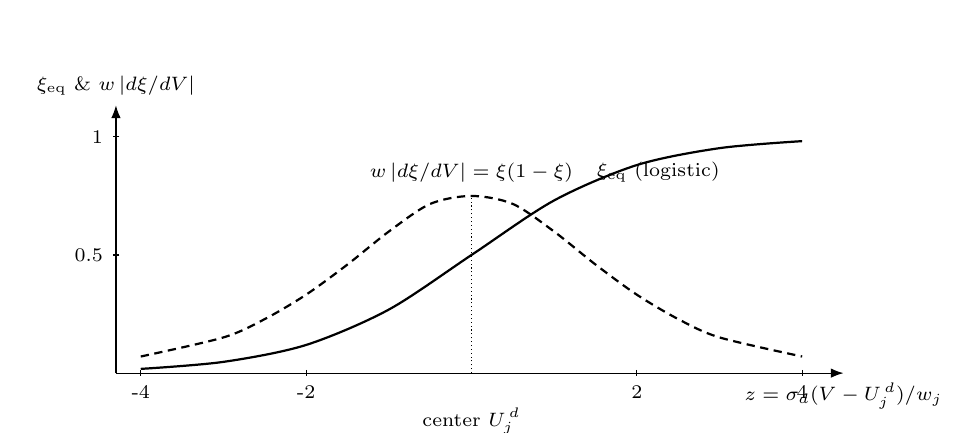
\begin{tikzpicture}[x=1.05cm,y=1.0cm]
% left axis: xi_eq (S-curve), right: dxi/dV bell -- shared z-axis
\draw[-{Latex[length=1.6mm]}] (-4.3,0) -- (4.5,0) node[below,font=\scriptsize] {$z=\sigma_d(V-U_j^{\,d})/w_j$};
\draw[-{Latex[length=1.6mm]}] (-4.3,0) -- (-4.3,3.4) node[above,font=\scriptsize] {$\xi_\eq$ \&\ $w\,|d\xi/dV|$};
\foreach \xx in {-4,-2,2,4} {\draw (\xx,0.04) -- (\xx,-0.04) node[below,font=\scriptsize] {\xx};}
\draw (-4.26,3.0) -- (-4.34,3.0) node[left,font=\scriptsize] {1};
\draw (-4.26,1.5) -- (-4.34,1.5) node[left,font=\scriptsize] {0.5};
% xi_eq = 1/(1+e^-z) scaled by 3
\draw[thick] plot[smooth] coordinates {(-4,0.0537) (-3,0.1429) (-2,0.3577) (-1,0.8068) (0,1.5) (1,2.1932) (2,2.6423) (3,2.8571) (4,2.9463)};
\node[right,font=\scriptsize] at (1.4,2.55) {$\xi_\eq$ (logistic)};
% derivative xi(1-xi) max 0.25 scaled by 12 -> max 3
\draw[densely dashed,thick] plot[smooth] coordinates {(-4,0.211) (-3,0.4534) (-2.5,0.6864) (-2,0.9963) (-1.5,1.3792) (-1,1.7976) (-0.5,2.1487) (0,2.25) (0.5,2.1487) (1,1.7976) (1.5,1.3792) (2,0.9963) (2.5,0.6864) (3,0.4534) (4,0.211)};
\node[font=\scriptsize] at (0,2.55) {$w\,|d\xi/dV|=\xi(1-\xi)$};
\draw[densely dotted] (0,0)--(0,2.25);
\node[below,font=\scriptsize] at (0,-0.32) {center $U_j^{\,d}$};
\end{tikzpicture}
\caption{평형 점유와 그 미분(v7-11 유래). 실선 $=\xi_\eq$ logistic(식~\eqref{eq:xieq}), 파선 $=$ 폭으로 규격화한 미분
$w_j|d\xi_\eq/dV|=\xi_\eq(1-\xi_\eq)$ — $z=0$(중심 $U_j^{\,d}$)에서 최대 $\tfrac14$ 인 종 모양. 이 종이
다음 절의 평형 peak 이고, 방향에 불변(양수)이다.}
\label{fig:logistic}
\end{figure}

% ====================================================================
\section{평형 peak — $|I|\to0$ 기준선 (N6)}\label{sec:eqpeak}
% ====================================================================
코드는 평형 점유에서 곧바로 평형 peak 모양 $\xi_\eq(1-\xi_\eq)/w$ 를 만든다. 이것이 전류가 없을 때($|I|\to0$)의
기준선이며, 동역학 꼬리가 무시될 만큼 작을 때 코드가 직접 쓰는 항이다.

\subsection{전하 보존과 logistic 미분}
관측 $\dd Q/\dd V$ 는 전하 보존식 $Q_\cell q=Q_\bg(V_n)+\sum_jQ_j\xi_j$ 를 궤적 $q$ 로 미분해
$\dd Q/\dd V_n=C_\bg+\sum_jQ_j\,\dd\xi_j/\dd V_n$ 으로 닫힌다. 평형 추종이면 $\dd\xi_j/\dd V_n$ 에 평형 기울기가 들어온다.

\begin{derivebox}
\textbf{출발: logistic 항등식.} $\xi_\eq=(1+e^{-z})^{-1}$, $z\equiv\sigma_d(V-U_j^{\,d})/w_j$ 를 $z$ 로 미분하면:
\begin{equation*}
\frac{\dd\xi_\eq}{\dd z}=\frac{e^{-z}}{(1+e^{-z})^2}=\frac{1}{1+e^{-z}}\cdot\frac{e^{-z}}{1+e^{-z}}=\xi_\eq(1-\xi_\eq).
\end{equation*}
\textbf{연쇄율 적용.} $\dd z/\dd V=\sigma_d/w_j$ 이므로:
\begin{equation*}
\frac{\dd\xi_{\eq,j}}{\dd V}=\frac{\dd\xi_\eq}{\dd z}\cdot\frac{\dd z}{\dd V}=\xi_\eq(1-\xi_\eq)\cdot\frac{\sigma_d}{w_j}.
\end{equation*}
\textbf{중간식 — 절댓값.} $\sigma_d=\pm1$ 이라 $|\dd\xi_\eq/\dd V|=\xi_\eq(1-\xi_\eq)/w_j$ (부호 불변, 양수).
\end{derivebox}

따라서 전이 $j$ 의 평형 peak 기여는
\begin{equation}
\frac{\dd\xi_{\eq,j}}{\dd V}=\frac{\sigma_d\,\xi_{\eq,j}(1-\xi_{\eq,j})}{w_j}
\;\Longrightarrow\;
\boxed{\;\Big(\frac{\dd Q}{\dd V}\Big)^\eq_j
=Q_j\,\frac{\xi_{\eq,j}(1-\xi_{\eq,j})}{w_j}
=Q_j\,\Big|\frac{\dd\xi_{\eq,j}}{\dd V}\Big|\;.}
\label{eq:eqpeak}
\end{equation}
이것이 코드의 \code{peak\_shape = ksi\_eq * (1 - ksi\_eq) / w} 이며, 메서드 \code{equilibrium} 이 전이별로 이 항만
합산한 것($C_\bg+\sum_jQ_j\xi_\eq(1-\xi_\eq)/w$)이다.

\textbf{부호.} $\sigma_d$ 가 미분에서 한 번 들어오지만 peak 모양은
절댓값 $|\dd\xi/\dd V|=\xi_\eq(1-\xi_\eq)/w$ 로 양수이고 방향 불변이다. 세 양 — 위치 $=$ 중심
$U_j^{\,d}$, 순높이 $=Q_j/(4w_j)$($\xi=\tfrac12$ 에서 $\xi(1-\xi)=\tfrac14$), 배경 차감 면적 $=Q_j$ —
가 이 한 식에서 읽힌다.

% ====================================================================
\section{동역학 지연 길이 $L_V$ (N7)}\label{sec:lag}
% ====================================================================
유한 전류에서는 평형 목표 $\xi_\eq$ 를 점유가 즉시 따라가지 못하고 뒤처진다 — 그 지연이 peak 의 꼬리다.
이 절은 사슬 $\mathcal A\to\chi_d\to\Delta H_a^\eff\to L_q\to L_V$ 를 단계별로 닫는다.

\subsection{지연의 보편 방정식과 용량축 길이 $L_q$}
정전류에서 $\dd q/\dd t=|I|/Q_\cell$ 이다.

\begin{derivebox}
\textbf{출발: 운동방정식.} $\dd\xi_j/\dd t=k_j(\xi_{\eq,j}-\xi_j)$.

\textbf{시간 $\to$ 용량 축 전환.} 양변을 $\dd q/\dd t=|I|/Q_\cell$ 로 나누면:
$\dd\xi_j/\dd q=(Q_\cell k_j/|I|)(\xi_{\eq,j}-\xi_j)$.

\textbf{지연 $r_j\equiv\xi_{\eq,j}-\xi_j$ 의 방정식.}
$\dd r_j/\dd q=\dd\xi_{\eq,j}/\dd q-\dd\xi_j/\dd q=\dd\xi_{\eq,j}/\dd q-(Q_\cell k_j/|I|)(\xi_{\eq,j}-\xi_j)$
$=\dd\xi_{\eq,j}/\dd q-r_j/L_{q,j}$.
\end{derivebox}

\begin{equation}
\frac{\dd r_j}{\dd q}=\frac{\dd\xi_{\eq,j}}{\dd q}-\frac{r_j}{L_{q,j}},
\qquad L_{q,j}=\frac{|I|}{Q_\cell\,k_j}.
\label{eq:Lq}
\end{equation}
$L_{q,j}$ 는 요구($|I|/Q_\cell$)와 공급($k_j$) 의 비 그 자체다.

\textbf{완화 속도 $k_j$.} detailed balance $k^-/k^+=e^{-\mathcal A_j/RT}$ 에서 $k_j=k^++k^-=k^+(1+e^{-\mathcal A_j/RT})$.

\subsection{컷 affinity $\mathcal A$ — 꼬리 시작점의 구동력}
$L_q$ 는 전이당 한 점(꼬리 컷점 $q_a$)에서 상수로 동결된다. 컷점은 원천 $\dd\xi_\eq/\dd q$ 가 정점의
약 $5\%$ 로 떨어지는 좌표이고, 그곳의 구동력을 $\mathcal A$ 로 정한다:

\begin{derivebox}
\textbf{logistic 미분의 $5\%$ 조건.} $\xi_\eq(1-\xi_\eq)/w=0.05\cdot(1/4)/w$ 에서 $\xi_\eq(1-\xi_\eq)=0.0125$.
logistic 에서 $\xi(1-\xi)=e^{-z}/(1+e^{-z})^2\approx e^{-z}$ ($z\gg0$) 이면 $e^{-z}=0.0125$, 즉 $z\approx4.357=z_\mathrm{cut}$.
구동력 $\mathcal A=z_\mathrm{cut}\cdot n_jRT$ (폭 다중도 포함).
\end{derivebox}

\begin{equation}
\mathcal A=\min\!\big(z_\mathrm{cut}\,n_j\,RT,\;A_\mathrm{cap}\,RT\big),
\qquad z_\mathrm{cut}=4.357,\ A_\mathrm{cap}=4.0\ (\text{기본}).
\label{eq:Acut}
\end{equation}
이것이 코드의 \code{A = min(z\_cut * n\_safe * R*T, A\_cap * R*T)} 다. $\mathcal A$ 의 크기는 충$\cdot$방전
동일($n_j>0$ 라 항상 양수)이고, 방향은 아래 $\chi_d\cdot\Delta H_a^\eff$ 가 받는다.

\subsection{방향별 전달 계수와 유효 장벽}
전이상태가 정$\cdot$역 장벽을 비대칭으로 가르는 분율 $\chi\in[0,1]$ 의 합-1 제약($\chi+\chi'=1$,
detailed balance)에서, 방향별 전달 계수는
\begin{equation}
\chi_d=\chi_\mathrm{split}(\chi,\sigma_d)=
\begin{cases}\chi & \sigma_d\ge0\ (\text{방전})\\ 1-\chi & \sigma_d<0\ (\text{충전}).\end{cases}
\label{eq:chid}
\end{equation}
깊은 꼬리에서 방전은 $\xi\to1$, 충전은 $\xi\to0$ 거울이라 역방향 장벽의 상수 몫이 같은 $+\Omega$ 로 흡수되는 것을 반영한다.

\begin{derivebox}
\textbf{유효 장벽.} 깊은 꼬리($\xi\to1$, 방전)에서 상호작용 몫 $\Omega(1-2\xi)\to-\Omega$ 가 역방향 장벽에
더해진다. 이를 활성화 엔탈피에 흡수하면: $\Delta H_a^\eff=\Delta H_a-\chi_d\cdot\Omega$. (충전 $\chi_d=1-\chi$,
$\xi\to0$ 에서 $\Omega(1-2\xi)\to+\Omega$, 정방향 장벽에 $-(1-\chi)\Omega$ 하강, 같은 방향 정합.)
\end{derivebox}

\begin{equation}
\boxed{\;\Delta H_{a,j}^\eff=\Delta H_{a,j}-\chi_d\,\Omega_j\;.}
\label{eq:dHeff}
\end{equation}

\subsection{$L_q$ 의 평가와 전압축 환산 $L_V$}
$k_j=k^+(1+e^{-\mathcal A_j/RT})$ 와 $k^+\simeq k_0 e^{-(\Delta G_a^\eff-\chi_d\mathcal A)/RT}$ ($k_0=k_BT/h$)를
식~\eqref{eq:Lq} 에 넣는다:

\begin{derivebox}
\textbf{출발:} $L_{q,j}=|I|/(Q_\cell k_j)$.

\textbf{$k_j$ 대입:} $k_j=k_0 e^{-(\Delta G_a^\eff-\chi_d\mathcal A)/RT}(1+e^{-\mathcal A/RT})$.
$k_0=k_BT/h$ 이므로 $T_*\equiv|I|h/(Q_\cell k_B)$ 로 정의하면:
\begin{equation*}
L_{q,j}=\frac{|I|}{Q_\cell}\cdot\frac{h}{k_BT}\cdot\frac{e^{(\Delta G_a^\eff-\chi_d\mathcal A)/RT}}{1+e^{-\mathcal A/RT}}
=\frac{T_*}{T}\cdot\frac{e^{(\Delta H_a^\eff-T\Delta S_a)/RT}}{1+e^{-\mathcal A/RT}}\cdot e^{-\chi_d\mathcal A/RT}.
\end{equation*}
\textbf{중간식 — 로그 형태:}
$\ln L_{q,j}=\ln(T_*/T)-\ln(1+e^{-\mathcal A/RT})+(\Delta H_a^\eff-T\Delta S_a)/RT-\chi_d\mathcal A/RT$.
\end{derivebox}

\begin{equation}
L_{q,j}=\frac{T_*}{T}\,\frac{\exp\!\big[(\Delta H_{a,j}^\eff-T\Delta S_{a,j})/RT\big]}{1+e^{-\mathcal A/RT}}
\,e^{-\chi_d\mathcal A/RT},
\qquad T_*\equiv\frac{|I|\,h}{Q_\cell\,k_B}.
\label{eq:Lqfull}
\end{equation}
전압축으로 옮기면 컷점 OCV 기울기를 곱한다:
\begin{equation}
\boxed{\;L_{V,j}=\Big|\frac{\dd V}{\dd q}\Big|_{q_a}\,L_{q,j}\;=\;|\code{dVdq\_qa}|\cdot L_{q,j}\;.}
\label{eq:LV}
\end{equation}
코드의 \code{return abs(dVdq\_qa) * L\_q} 다.

\textbf{컷 부등식의 지위.} $\mathcal A$ 가 전이당 컷 상수이므로, 코드 안에서 $L_q$ 는 $V$ 의 함수로 다시 미분되지 않는다:
\emph{운영상 실현 미분 $\partial\ln L_q/\partial V=0$.} 부등식 $\partial\ln L_q/\partial V<0$ 은 컷 규칙의 \emph{물리적 동기}로만 성립한다 — 국소 구동력으로 두면
$V\!\uparrow\Rightarrow\mathcal A\!\uparrow\Rightarrow$ 유효 장벽$\downarrow\Rightarrow L_q\downarrow$ 임을 가리킨다.

\begin{codebox}
\textbf{N7 진행.} \code{n\_safe=|n\_j|} $\to$ $\mathcal A$(식~\eqref{eq:Acut}) $\to$
\code{(chi\_d, dH\_a\_use)=\_chi\_and\_dH\_eff(...)} (식~\eqref{eq:chid}$\cdot$\eqref{eq:dHeff}) $\to$
\code{L\_q=func\_L\_q(...,x=chi\_d,A=A)} (식~\eqref{eq:Lqfull}) $\to$ \code{L\_V=|dVdq\_qa|*L\_q} (식~\eqref{eq:LV}).
전이당 \emph{상수}(대표 $T_\rep\cdot$대표 $n$)로 한 번 평가한다.
\end{codebox}

% ====================================================================
\section{인과 저역통과 꼬리 (N8)}\label{sec:tail}
% ====================================================================
$L_V$ 가 확보되면 코드는 평형 점유 $\xi_\eq$ 를 이 척도로 지수 완화시켜 실제 점유 $\xi_\lag$ 를 얻고,
$(\xi_\eq-\xi_\lag)/L_V$ 를 전류 보정 peak 로 합산에 넣는다.

\subsection{ODE 일반해와 이산 근사}
지연 ODE (식~\eqref{eq:Lq}) $\dd r/\dd q=\dd\xi_\eq/\dd q-r/L_q$ 를 전압축으로 바꾸면
$\dd r/\dd V=\dd\xi_\eq/\dd V-r/L_V$ 이다. 이것은 선형 1차 ODE 이므로 적분인자 $e^{V/L_V}$ 로 닫힌다:

\begin{derivebox}
\textbf{출발: } $\dfrac{\dd r}{\dd V}+\dfrac{r}{L_V}=\dfrac{\dd\xi_\eq}{\dd V}$.

\textbf{적분인자.} 양변에 $e^{V/L_V}$ 를 곱하면 좌변이 완전미분으로 묶인다:
\begin{equation*}
\frac{\dd}{\dd V}\!\big(r\,e^{V/L_V}\big)=e^{V/L_V}\frac{\dd\xi_\eq}{\dd V}.
\end{equation*}
\textbf{양변 $[V_0,V]$ 구간 적분:}
\begin{equation*}
r(V)=e^{-(V-V_0)/L_V}r(V_0)+\int_{V_0}^V e^{-(V-V')/L_V}\frac{\dd\xi_\eq}{\dd V'}\,\dd V'.
\end{equation*}
\textbf{중간식 — 이산 근사.} 균일 격자 $|\Delta V|=|V_{i+1}-V_i|$ 에서 $\rho\equiv e^{-|\Delta V|/L_V}$ 로 놓으면:
$\xi_{\lag,i+1}\approx\rho\,\xi_{\lag,i}+(1-\rho)\,\xi_{\eq,i}$.
\end{derivebox}

\begin{equation}
\boxed{\;\xi_{\lag}[i{+}1]=\rho\,\xi_{\lag}[i]+(1-\rho)\,\xi_{\eq}[i],
\qquad\rho=e^{-|\Delta V|/L_{V,j}}\;.}
\label{eq:lowpass}
\end{equation}
이것이 인과 저역통과다 — $\xi_\lag$ 는 미래 격자를 보지 않고 과거 $i$ 의 $\xi_\eq$ 만 끌어쓴다.

\subsection{충전 격자 역전 — 인과 방향 보정}
방전은 $V$ 가 단조 감소해 격자 $i=0\to N$ 이 시간 순방향과 일치하므로 식~\eqref{eq:lowpass} 를 그대로 적용한다. 충전은 $V$ 가 증가해 인과 방향이 반대다:

\begin{derivebox}
\textbf{인과 조건.} 저역통과의 "과거만 보기" 성질은 격자 인덱스 $i$ 가 시간 증가 방향을 향할 때 성립한다.
충전 $V\!\uparrow$: 격자 $i=0\to N$ 은 시간 역방향이므로 직접 적용하면 미래 $\xi_\eq$ 에 의존하는
반인과 필터가 된다.

\textbf{처방.} 충전 격자를 반전($[::-1]$)해 $V$ 가 단조 감소하는 순서로 바꾼 뒤 식~\eqref{eq:lowpass} 를 돌리고,
결과를 다시 반전한다.
\end{derivebox}

\begin{equation}
\boxed{\;\xi_\lag^\chg=\big[\,\text{lowpass}\!\big(\xi_\eq[::-1],\,\rho\big)\,\big][::-1]\;.}
\label{eq:reversal}
\end{equation}
코드의 \code{ksi\_eq\_rev = ksi\_eq[::-1]; ksi\_lag\_rev = lowpass(ksi\_eq\_rev, rho); ksi\_lag = ksi\_lag\_rev[::-1]}.

인과 꼬리 모양은
\begin{equation}
\mathrm{peak}_j^\tail=\frac{\xi_{\eq,j}-\xi_{\lag,j}}{L_{V,j}}.
\label{eq:peakshape}
\end{equation}
이것이 코드의 \code{peak\_shape = (ksi\_eq - ksi\_lag) / L\_V} 이다.

\begin{figure}[t]
\centering
\begin{tikzpicture}[x=1.15cm,y=3.2cm]
\draw[-{Latex[length=1.6mm]}] (0,0) -- (8.3,0) node[below,font=\scriptsize] {$V$ (discharge: $\rightarrow$ decreasing)};
\draw[-{Latex[length=1.6mm]}] (0,0) -- (0,1.55) node[left,font=\scriptsize] {$\xi$};
\draw[densely dotted] (4.0,0)--(4.0,1.1);
\node[below,font=\scriptsize] at (4.0,-0.08) {$U_j^d$};
% xi_eq S-curve (smoothed)
\draw[thick] plot[smooth] coordinates {(0.2,0.02)(0.5,0.03)(1.0,0.05)(1.5,0.09)(2.0,0.14)(2.5,0.21)(3.0,0.31)(3.5,0.42)(4.0,0.50)(4.5,0.58)(5.0,0.66)(5.5,0.75)(6.0,0.85)(6.5,0.92)(7.0,0.95)(7.5,0.97)};
\node[right,font=\scriptsize] at (7.6,0.97) {$\xi_\eq$};
% xi_lag lagged curve
\draw[densely dashed,thick] plot[smooth] coordinates {(0.2,0.02)(0.5,0.03)(1.0,0.04)(1.5,0.07)(2.0,0.10)(2.5,0.16)(3.0,0.24)(3.5,0.34)(4.0,0.43)(4.5,0.53)(5.0,0.62)(5.5,0.72)(6.0,0.83)(6.5,0.91)(7.0,0.94)(7.5,0.97)};
\node[right,font=\scriptsize] at (7.6,0.92) {$\xi_\lag$};
% lag gap annotation
\draw[{Latex[length=1.2mm]}-{Latex[length=1.2mm]}] (3.0,0.24) -- (3.0,0.31);
\node[left,font=\scriptsize,align=right] at (2.9,0.275) {$r=\xi_\eq-\xi_\lag$\\$\rightarrow$ tail peak};
\end{tikzpicture}
\caption{인과 저역통과 완화(v7-11 유래, 방전). 실선 $=\xi_\eq$, 파선 $=\xi_\lag$. 라그 $r=\xi_\eq-\xi_\lag$ 가
전위가 내려가는 방향(오른쪽)에 쌓이고 $r/L_V$ 가 꼬리 peak 다. 충전에서는 격자를 역전(식~\eqref{eq:reversal})해
같은 인과 필터를 적용한다.}
\label{fig:reversal}
\end{figure}

% ====================================================================
\section{합산 및 역보간 (N9)}\label{sec:sum}
% ====================================================================
모든 전이 루프가 닫힌 뒤, 보존식을 선형으로 합산하고 직류 분극 전위로 옮긴다.

\subsection{합산식}
\begin{equation}
\frac{\dd Q}{\dd V_n}\bigg|_\tot
=C_\bg+\sum_j Q_j\,\mathrm{peak}_j,
\qquad
\mathrm{peak}_j=
\begin{cases}
\sigma_d\,\dfrac{\xi_{\eq,j}(1-\xi_{\eq,j})}{w_j} & (\text{평형 모드})\\[4pt]
\dfrac{\xi_{\eq,j}-\xi_{\lag,j}}{L_{V,j}} & (\text{동역학 꼬리 모드}).
\end{cases}
\label{eq:sum}
\end{equation}

\subsection{직류 분극 전위 $V_n$}
피팅 전위는 측정 단자전압 $V_\app$ 에서 ohm 강하를 뺀 음극 전위 $V_n$ 이다:
\begin{equation}
\boxed{\;V_n=V_\app-\sigma_d\,|I|\,R_n\;.}
\label{eq:vn}
\end{equation}
방전($\sigma_d=+1$): 전류가 흘러 $V_\app>V_n$, 충전: $V_\app<V_n$. $R_n$ 은 음극 직류 저항.

\subsection{역보간}
$Q_\target$ 에 대응하는 $V_n$ 을 역보간으로 얻는다: 합산 $\dd Q/\dd V$ 를 누적하면 $Q(V)$ 가 나오고,
\code{np.interp(q\_target, Q\_cumsum[::-1], V\_grid[::-1])} 패턴으로 $V_n(q)$ 를 돌려준다.

% ====================================================================
\section*{부호 검산 (Sign Check)}\label{sec:signcheck}
% ====================================================================
\begin{signbox}
\begin{enumerate}[label=\textbf{S\arabic*.},leftmargin=*,itemsep=2pt]
\item \textbf{$U_j(T)$}: $U_j=(- \Delta H_{\rxn,j}+T\Delta S_{\rxn,j})/F$ — 흡열 전이는 $U_j$ 증가, 엔트로피 증가도 $U_j$ 증가. \checkmark
\item \textbf{logistic 방향}: 방전 $\sigma_d=+1$이면 $z=+(V-U)/w$, $V\!\uparrow\Rightarrow z\!\uparrow\Rightarrow\xi_\eq\!\uparrow$(탈리튬화 증가). 충전 $\sigma_d=-1$이면 $z=-(V-U)/w$, $V\!\uparrow\Rightarrow\xi_\eq\!\downarrow$(삽입 증가). \checkmark
\item \textbf{dQ/dV peak 양수}: 방향 불변 $|\dd\xi/\dd V|=\xi(1-\xi)/w\ge0$, 부호는 $Q_j>0$ 이 보장. \checkmark
\item \textbf{$\Delta U_j^\hys\ge0$}: $u_j\in[0,1)$, $\Omega_j u_j\ge2RT\,\mathrm{artanh}\,u_j$ 임을 $f(u)=\Omega u-2RT\,\mathrm{artanh}\,u|_{u\to0}\to0, f'>0$ 으로 확인. $\Omega_j\le2RT$이면 $u_j$ 허수 $\Rightarrow$ 코드 0 반환. \checkmark
\item \textbf{분기 $\pm\frac12\sigma_d\gamma\Delta U^\hys$}: 방전 $\sigma_d=+1$이면 $U^d>U_j$(높은 전위 과주행), 충전이면 $U^d<U_j$. 방전 dQ/dV peak가 충전 peak보다 오른쪽(높은 $V$). \checkmark
\item \textbf{$\chi_d$ 합-1}: 방전 $\chi_d=\chi$, 충전 $\chi_d=1-\chi$, 합 $=1$. detailed balance $k^-/k^+=e^{-\mathcal A/RT}$ 보존. \checkmark
\item \textbf{$\Delta H_a^\eff=\Delta H_a-\chi_d\Omega$}: 깊은 꼬리서 상호작용이 장벽을 낮추는 방향 흡수. 부호: $\Omega>0$이면 유효 장벽 하강 $\Rightarrow k_j\uparrow\Rightarrow L_q\downarrow$(빠른 완화). 물리적으로 일관. \checkmark
\item \textbf{운영 $\partial\ln L_q/\partial V=0$}: $\mathcal A$ 는 전이당 컷 상수 — $V$ 따라 변하지 않음. 부등식 $\partial\ln L_q/\partial V<0$ 은 컷 선택 동기이지 실행 미분 아님. \checkmark
\end{enumerate}
\end{signbox}

% ====================================================================
\section{표 — 스테이징·입력·노드맵}\label{sec:tables}
% ====================================================================

\begin{table}[ht]
\centering
\caption{흑연 스테이징 전이 목록 (Stage $4\!\to\!3\!\to\!2L\!\to\!2\!\to\!1$).\label{tab:staging}}
\small
\begin{tabular}{@{}lcccc@{}}
\toprule
전이 ID & 스테이지 변화 & $U_j$ 근사값 (V) & 비고\\
\midrule
T1 & $4\!\to\!3$ & 0.210 & 저용량 피크\\
T2 & $3\!\to\!2L$ & 0.120 & 2L 준결정\\
T3 & $2L\!\to\!2$ & 0.090 & 메인 피크 전\\
T4 & $2\!\to\!1$ & 0.075 & 메인 피크 (가장 큰 $Q_j$)\\
\bottomrule
\end{tabular}
\end{table}

\begin{table}[ht]
\centering
\caption{주요 입력 파라미터 목록.\label{tab:inputs}}
\small
\begin{tabular}{@{}llll@{}}
\toprule
기호 & 의미 & 단위 & 코드 키\\
\midrule
$U_j$ & 평형 전위 중심 & V & \code{U}\\
$n_j$ & 폭 다중도 & -- & \code{n}\\
$Q_j$ & 전이 용량 & Ah & \code{Q}\\
$\Omega_j$ & 정규용액 상호작용 에너지 & J/mol & \code{Omega}\\
$\gamma_j$ & 분기 인자 ($\le1$) & -- & \code{gamma}\\
$\chi$ & 전달 계수 & -- & \code{chi}\\
$\Delta H_a$ & 활성화 엔탈피 & J/mol & \code{dHa}\\
$\Delta S_a$ & 활성화 엔트로피 & J/(mol$\cdot$K) & \code{dSa}\\
$C_\bg$ & 배경 용량 & F & \code{C\_bg}\\
$R_n$ & 음극 직류 저항 & $\Omega$ & \code{Rn}\\
\bottomrule
\end{tabular}
\end{table}

\begin{table}[ht]
\centering
\caption{N0–N9 코드 노드 맵.\label{tab:nodemap}}
\small
\begin{tabular}{@{}lll@{}}
\toprule
노드 & 주요 출력 & 핵심 식\\
\midrule
N0 & $V_n$ 격자, 방향 $\sigma_d$ & 식~\eqref{eq:vn}\\
N1 & 전이 루프 개시 & ---\\
N2 & $U_j^{\,d}$ (분기 중심) & 식~\eqref{eq:Uj}, \eqref{eq:Ubranch}\\
N3 & $\Delta U_j^\hys$, $U_j^{\,d}$ & 식~\eqref{eq:spinodal}, \eqref{eq:dUhys}\\
N4 & $w_j$ & 식~\eqref{eq:wbase}\\
N5 & $\xi_{\eq,j}$ & 식~\eqref{eq:xieq}\\
N6 & 평형 peak & 식~\eqref{eq:eqpeak}\\
N7 & $L_{q,j}$, $L_{V,j}$ & 식~\eqref{eq:Acut}, \eqref{eq:dHeff}, \eqref{eq:Lqfull}, \eqref{eq:LV}\\
N8 & $\xi_{\lag,j}$, 꼬리 peak & 식~\eqref{eq:lowpass}, \eqref{eq:reversal}, \eqref{eq:peakshape}\\
N9 & 합산, $Q(V)$, 역보간 & 식~\eqref{eq:sum}\\
\bottomrule
\end{tabular}
\end{table}

% ====================================================================
\begin{thebibliography}{9}
\bibitem{dahn1991} J.\,R.\ Dahn, ``Phase diagram of $\mathrm{Li}_x\mathrm{C}_6$,'' \textit{Phys.\ Rev.\ B} \textbf{44}, 9170 (1991).
\bibitem{ohzuku1993} T.\ Ohzuku, Y.\ Iwakoshi, K.\ Sawai, ``Formation of lithium-graphite intercalation compounds in nonaqueous electrolytes,'' \textit{J.\ Electrochem.\ Soc.} \textbf{140}, 2490 (1993).
\bibitem{bloom2005} I.\ Bloom \textit{et al.}, ``Differential voltage analyses of high-power, lithium-ion cells,'' \textit{J.\ Power Sources} \textbf{139}, 295 (2005).
\bibitem{dubarry2012} M.\ Dubarry, B.\,Y.\ Liaw, ``Identify capacity fading mechanism in a commercial LiFePO$_4$ cell,'' \textit{J.\ Power Sources} \textbf{194}, 541 (2009).
\bibitem{bard2001} A.\,J.\ Bard, L.\,R.\ Faulkner, \textit{Electrochemical Methods}, 2nd ed.\ (Wiley, 2001).
\bibitem{eyring1935} H.\ Eyring, ``The Activated Complex in Chemical Reactions,'' \textit{J.\ Chem.\ Phys.} \textbf{3}, 107 (1935).
\bibitem{newmann2004} J.\ Newman, K.\,E.\ Thomas-Alyea, \textit{Electrochemical Systems}, 3rd ed.\ (Wiley, 2004).
\end{thebibliography}

\end{document}
